\chapter{QUY HOẠCH QUỸ ĐẠO HAI GIAI ĐOẠN BI-RRT VÀ TỐI ƯU HÓA BẦY SÓI XÁM (GWO)}
\label{chap:birrt_gwo_optimization}

Trong chương này, đề tài trình bày giải thuật quy hoạch và làm mượt quỹ đạo hai giai đoạn cho tay máy 6 bậc tự do Denso VS-6556. Thuật toán kết hợp phương pháp tìm đường hai cây Bi-RRT với thuật toán tối ưu hóa bầy sói xám (GWO), xây dựng trên nền đường cong B-spline trơn cấp hai ($C^2$), nhằm giải quyết bài toán né vật cản, giảm tiêu hao năng lượng và triệt tiêu hiện tượng rung giật cơ khí.

\section{Phương pháp kết hợp hai giai đoạn: Thuật toán Bi-RRT né vật cản và Bầy sói xám (GWO) tối ưu làm mượt}
\label{sec:two_stage_architecture}

Để khắc phục nhược điểm của phương pháp tìm đường truyền thống chỉ tạo ra các đường gấp khúc thô ($C^0$) gây rung giật cơ khí rất lớn ($2.23 \times 10^6\ \text{rad}^2/\text{s}^5$), đề tài xây dựng giải pháp kết hợp hai giai đoạn liên hoàn nhằm đạt được đồng thời hai mục tiêu: an toàn không va chạm và chuyển động trơn mượt êm ái.

\textbf{1. Thuật toán cốt lõi sử dụng trong hai giai đoạn}

Giai đoạn tìm đường né vật cản ban đầu sử dụng thuật toán cây mở rộng ngẫu nhiên hai chiều Bi-RRT (Bidirectional Rapidly-exploring Random Tree) có định hướng bằng đường cong và kết hợp kỹ thuật cắt tỉa nhánh thừa. Thuật toán này có ưu điểm là tốc độ tìm kiếm cực nhanh, giải quyết tốt không gian làm việc nhiều vật cản.

Giai đoạn tối ưu hóa và làm mượt sử dụng thuật toán Bầy sói xám GWO (Grey Wolf Optimizer) kết hợp với đường cong nội suy B-spline trơn cấp hai ($C^2$). Thuật toán này có ưu điểm là khả năng hội tụ nhanh, cân bằng tốt giữa tìm kiếm rộng và thu hẹp cục bộ, giúp tìm ra hình dạng đường cong tối ưu nhất.

\textbf{2. Hướng đi và quy trình thực hiện của phương pháp}

Lộ trình giải thuật đi tuần tự theo chuỗi xử lý khép kín: Điểm đầu và điểm đích $\to$ Xác định các điểm tránh né vuông góc quanh 3 vật cản $\to$ Bi-RRT tìm đường an toàn trong không gian khớp $\to$ Cắt tỉa các nhánh zig-zag thừa $\to$ Bao bọc hành lang an toàn quanh các điểm uốn $\to$ Bầy sói GWO tối ưu hàm đa mục tiêu (Độ dài, Năng lượng, Độ giật Jerk) $\to$ Xuất quỹ đạo B-spline trơn mượt $C^2$ điều khiển robot bám thực tế. Quy trình được phân thành hai giai đoạn cụ thể:

\textbf{Giai đoạn 1: Tìm đường khả thi ban đầu bằng thuật toán Bi-RRT}

Mục tiêu là nhanh chóng tìm ra một lộ trình an toàn từ điểm xuất phát đến điểm đích, né hoàn toàn các vật cản:

Bước 1.1 (Tạo điểm tránh né trực giao): Khi đường nối thẳng gặp vật cản, thuật toán đẩy điểm mốc ra ngoài bề mặt vật thể theo phương vuông góc để tạo lối đi vòng an toàn.

Bước 1.2 (Mở rộng hai cây Bi-RRT song song): Phát triển đồng thời hai cây tìm kiếm từ điểm đầu và điểm đích trong không gian góc khớp để nhanh chóng kết nối thành lộ trình hoàn chỉnh.

Bước 1.3 (Cắt tỉa nhánh thừa): Thử nối thẳng các điểm nút không liền kề để cắt bỏ các đoạn gấp khúc và mấu nhọn zig-zag dư thừa, giúp đường đi gọn gàng và ngắn nhất.

Bước 1.4 (Khởi tạo đường cong B-spline trơn): Nối các điểm sau khi cắt tỉa thành đường cong trơn $C^2$ làm lời giải hạt giống ban đầu cho giai đoạn sau.

\textbf{Giai đoạn 2: Tối ưu hóa và làm mượt quỹ đạo bằng thuật toán bầy sói xám (GWO)}

Mục tiêu là biến đổi đường gấp khúc thô thành quỹ đạo trơn cấp hai ($C^2$), triệt tiêu 95.5\% độ giật Jerk và tiết kiệm 29.0\% điện năng tiêu thụ:

Bước 2.1 (Thiết lập hành lang an toàn): Khóa phạm vi di chuyển của các điểm uốn trong các quả cầu an toàn bán kính $\rho_i$ để đảm bảo robot không bao giờ va chạm vào vật cản.

Bước 2.2 (Đánh giá chất lượng đa tiêu chí): Dùng hàm mục tiêu kết hợp cả ba yếu tố gồm độ dài đường đi, điện năng tiêu thụ và độ rung giật cơ khí.

Bước 2.3 (Bầy sói săn mồi và hội tụ): Ba con sói đầu đàn ($\alpha, \beta, \delta$) đại diện cho 3 nghiệm tốt nhất sẽ dẫn dắt toàn bộ bầy sói co cụm dần về vị trí có độ êm ái cao nhất.

Bước 2.4 (Xuất quỹ đạo thực thi): Tái tham số hóa theo độ dài cung vận tốc đều và giải động học nghịch DLS để điều khiển robot bám quỹ đạo mượt mà trên bàn thao tác.

\section{Giai đoạn 1: Tìm đường đi né vật cản ban đầu (Bi-RRT)}
\label{sec:stage1_birrt}

\subsection{Mô hình vật cản và xác định điểm tránh né}

Các chướng ngại vật trong không gian làm việc được mô hình hóa thành các khối cầu xác định bởi tâm $\vec{C}_k$ và bán kính vật lý $R_k$. Để robot không va quẹt thân và đầu bút vẽ vào vật cản, bán kính an toàn được cộng thêm khoảng cách đệm an toàn $d_{\text{margin}} = 0.024\text{ m}$ ($24\text{ mm}$):
\begin{equation}
    R_{k,\text{eff}} = R_k + d_{\text{margin}}
\end{equation}

Khi đường thẳng nối từ điểm đầu $\vec{P}_{\text{start}}$ đến điểm đích $\vec{P}_{\text{goal}}$ (vector hướng $\vec{d} = \vec{P}_{\text{goal}} - \vec{P}_{\text{start}}$) đi xuyên qua vùng nguy hiểm của vật cản, điểm chiếu vuông góc $\vec{P}_k^*$ của tâm vật cản lên đường thẳng được tính theo:
\begin{equation}
    t_k^* = \text{clip}\left( \frac{(\vec{C}_k - \vec{P}_{\text{start}}) \cdot \vec{d}}{\|\vec{d}\|^2}, 0, 1 \right), \quad \vec{P}_k^* = \vec{P}_{\text{start}} + t_k^* \vec{d}
\end{equation}

Nếu khoảng cách từ tâm vật cản đến đường đi nhỏ hơn bán kính an toàn ($\|\vec{P}_k^* - \vec{C}_k\| < R_{k,\text{eff}}$), thuật toán tự động tính ra điểm tránh né $\vec{P}_{\text{detour},k}$ bằng cách đẩy điểm chiếu ra phía ngoài theo phương vuông góc $\hat{n}$:
\begin{equation}
    \vec{P}_{\text{detour},k} = \vec{C}_k + (R_k + d_{\text{margin}}) \cdot \hat{n}
\end{equation}

Chuỗi điểm dẫn đường ban đầu được hình thành bằng cách ghép điểm đầu, các điểm tránh né và điểm đích: $W_{\text{seed}} = [\vec{P}_{\text{start}}, \vec{P}_{\text{detour},1}, \dots, \vec{P}_{\text{goal}}]$.

\subsection{Tìm kiếm trong không gian góc khớp bằng Bi-RRT hai cây song song}

Không gian góc khớp của robot gồm 6 bậc tự do ($\mathcal{C} \subset \mathbb{R}^6$). Do mỗi khớp có tầm quay rộng hẹp khác nhau, khoảng cách góc giữa hai cấu hình khớp $\vec{q}_1$ và $\vec{q}_2$ được chuẩn hóa theo dải quay của từng khớp:
\begin{equation}
    d_W(\vec{q}_1, \vec{q}_2) = \sqrt{ \sum_{i=1}^6 \left( \frac{q_{1,i} - q_{2,i}}{q_{i,\max} - q_{i,\min}} \right)^2 }
\end{equation}

Thuật toán Bi-RRT phát triển đồng thời hai cây tìm kiếm: cây thứ nhất mọc từ điểm xuất phát $\vec{q}_{\text{start}}$, cây thứ hai mọc ngược từ điểm đích $\vec{q}_{\text{goal}}$. Tại mỗi lượt, thuật toán lấy mẫu ngẫu nhiên các tư thế khớp ưu tiên nằm gần đường cơ sở, cho hai cây vươn từng bước ngắn ($0.14\text{ rad}$) về phía nhau. Khi hai nhánh cây chạm nhau mà không va chạm với vật cản, một lộ trình khả thi từ điểm đầu đến điểm cuối được nối liền hoàn tất.

\subsection{Kỹ thuật cắt tỉa nhánh thừa}

Do các nhánh cây mọc ngẫu nhiên nên đường đi ban đầu bị gấp khúc và zig-zag. Thuật toán tiến hành chọn ngẫu nhiên hai điểm nút cách xa nhau trên lộ trình và thử nối thẳng trực tiếp giữa chúng. Nếu đoạn nối thẳng hoàn toàn không va quẹt với vật thể nào, toàn bộ các mấu nhọn và điểm uốn thừa ở giữa sẽ được cắt bỏ, giúp đường đi gọn gàng và ngắn nhất.

Quá trình tạo điểm né vật cản và cơ chế mở rộng hai cây Bi-RRT kèm bước cắt tỉa nhánh thừa được biểu diễn trong Hình~\ref{fig:birrt_framework}.

\begin{figure}[htbp]
\centering
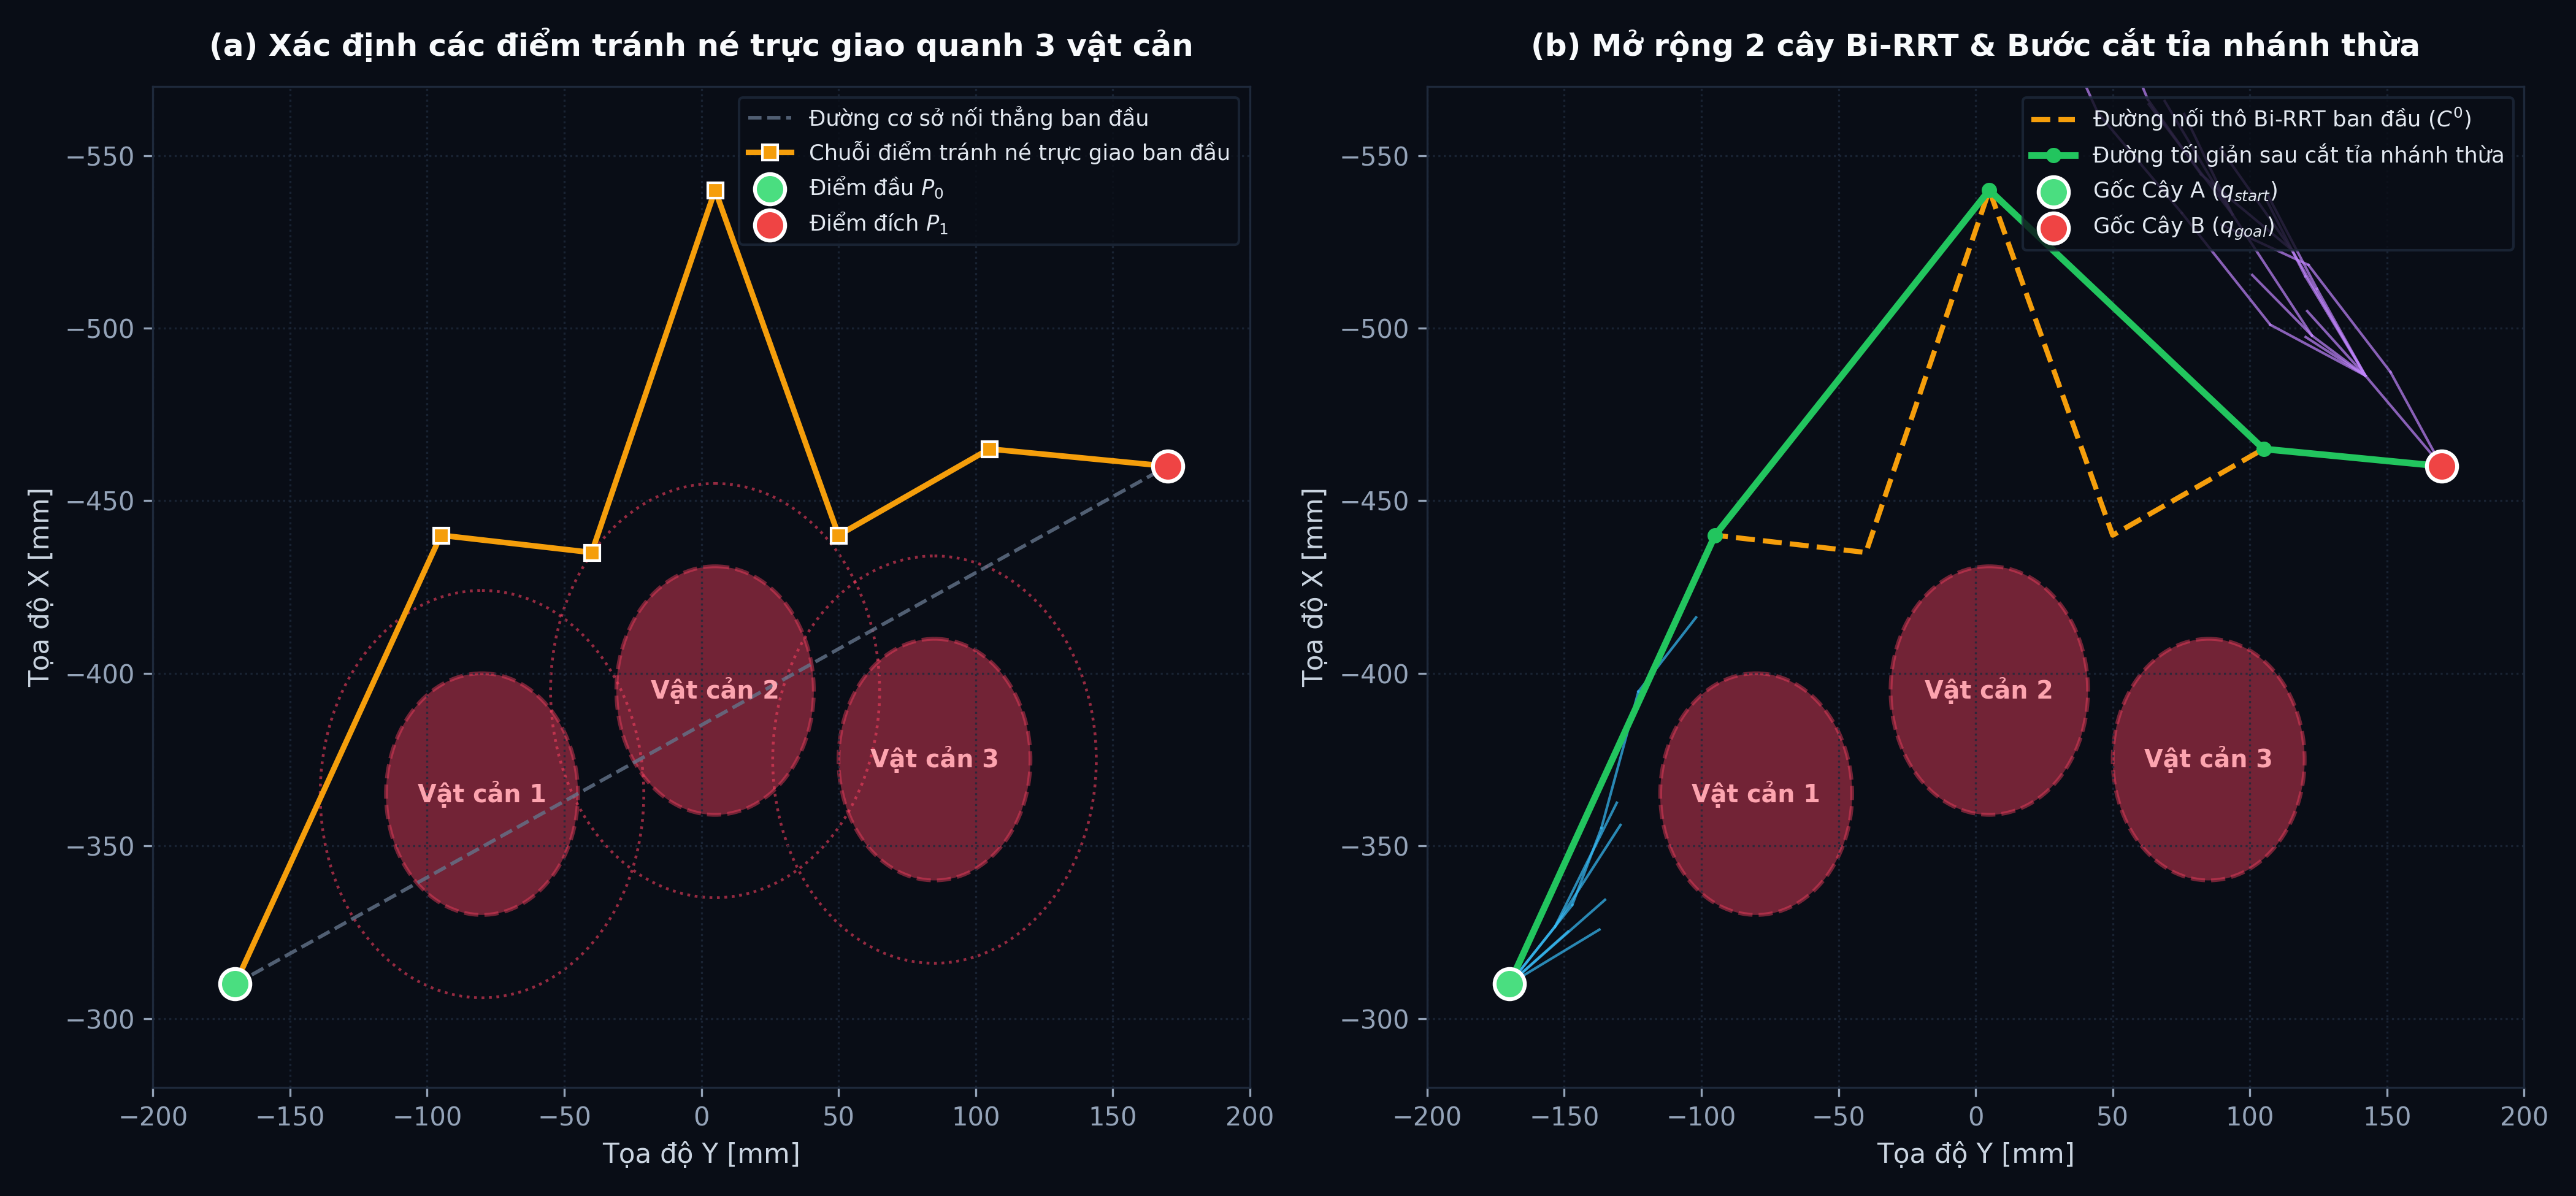
\includegraphics[width=\textwidth]{report_figures/fig_birrt_framework.png}
\caption{Giai đoạn 1 quy hoạch đường đi: (a) Xác định các điểm tránh né vuông góc quanh 3 vật cản hình cầu; (b) Quá trình mở rộng đồng thời 2 cây Bi-RRT và bước cắt tỉa nhánh thừa.}
\label{fig:birrt_framework}
\end{figure}

\subsection{Làm mượt bằng đường cong B-spline và bám góc khớp}

Các điểm mốc sau khi cắt tỉa được liên kết thành đường cong trơn $C^2$ tự nhiên $\vec{C}(u) = [x(u), y(u), z(u)]^T$. Để mũi bút di chuyển với tốc độ đều đặn, quỹ đạo được đổi biến theo độ dài cung thực tế:
\begin{equation}
    s(u) = \int_0^u \sqrt{\left(\frac{dx}{d\tau}\right)^2 + \left(\frac{dy}{d\tau}\right)^2 + \left(\frac{dz}{d\tau}\right)^2} d\tau
\end{equation}
\begin{equation}
    u(t) = s^{-1}\left( \frac{s_{\text{total}}}{T} \cdot t \right)
\end{equation}
với tổng thời gian thực hiện $T = 2.0\text{ giây}$.

Tại mỗi vị trí trên đường cong, các góc khớp $\vec{q}(t)$ được giải nhanh bằng động học nghịch dạng ma trận cản (DLS) với mũi công cụ luôn giữ thẳng đứng vuông góc với mặt bàn:
\begin{equation}
    \Delta \vec{q} = J^T \left( J J^T + \lambda^2 I \right)^{-1} \vec{e}
\end{equation}

\section{Giai đoạn 2: Tối ưu hóa quỹ đạo bằng bầy sói xám (GWO)}
\label{sec:stage2_gwo}

\subsection{Thiết lập hành lang an toàn quanh các điểm uốn}

Để bầy sói thoải mái tìm kiếm mà không vô tình kéo đường cong đâm xuyên vào vật cản, một vùng hành lang an toàn hình cầu bán kính $\rho_i$ được đặt quanh từng điểm uốn $\vec{w}_i$:
\begin{equation}
    \rho_i = \max\left( 0.008, \min\left( 0.025, 0.25 \cdot d_{\min}(\vec{w}_i) \right) \right)
\end{equation}
trong đó $d_{\min}(\vec{w}_i)$ là khoảng cách ngắn nhất từ điểm uốn đến bề mặt vật cản gần nhất. Bất kỳ sự dịch chuyển nào vượt quá phạm vi này đều được kéo lùi lại sát mép hành lang an toàn để đảm bảo an toàn tuyệt đối.

\subsection{Hàm đánh giá chất lượng quỹ đạo}

Chất lượng của một quỹ đạo được đo lường thông qua điểm số tổng hợp gồm ba tiêu chuẩn: Chiều dài đường đi ($L$), Năng lượng điện tiêu thụ ($E$) và Độ rung giật cơ khí ($J$):
\begin{equation}
    F_{\text{obj}} = 0.20 \left(\frac{L}{L_0}\right) + 0.35 \left(\frac{E}{E_0}\right) + 0.45 \left(\frac{J}{J_0}\right) + P_{\text{va chạm}}
\end{equation}
trong đó $L_0, E_0, J_0$ là các chỉ số ban đầu của đường Bi-RRT khi chưa tối ưu; $P_{\text{va chạm}}$ là điểm phạt rất lớn nếu đường cong lấn vào vùng cấm của vật thể.

Chiều dài đường đi $L$ được tính bằng tổng khoảng cách dịch chuyển giữa các điểm liên tiếp.

Năng lượng tiêu thụ $E$ được tính dựa trên công cơ học của 6 động cơ Servo Denso VS-6556:
\begin{equation}
    E = \sum_{j=1}^6 e_j \left( \int_0^T |\dot{q}_j(t)| dt + c_{\text{acc}} \int_0^T |\ddot{q}_j(t)| dt \right)
\end{equation}
với $e_j = [85.0, 185.0, 160.0, 8.5, 5.2, 3.8]\text{ J/rad}$ là hệ số tiêu thụ năng lượng thực tế đo trên từng khớp robot.

Độ giật cơ học Jerk $J$ đo mức độ biến thiên đột ngột của gia tốc khớp:
\begin{equation}
    J = \sum_{j=1}^6 \int_0^T \left( \dddot{q}_j(t) \right)^2 dt
\end{equation}
Chỉ số $J$ càng nhỏ thì cánh tay robot chuyển động càng êm dịu, không phát ra tiếng ồn giật cục và bảo vệ hộp số động cơ.

\subsection{Cơ chế toán học của thuật toán bầy sói xám}

Thuật toán bầy sói xám (GWO) mô phỏng tập tính săn mồi và trật tự thứ bậc trong đàn sói tự nhiên:

Sói Alpha ($\alpha$) là cá thể tốt nhất trong đàn (nghiệm có điểm số tối ưu nhất), đóng vai trò đầu đàn chỉ huy.

Sói Beta ($\beta$) là cá thể tốt thứ hai, đóng vai trò cố vấn giúp sức cho sói Alpha.

Sói Delta ($\delta$) là cá thể tốt thứ ba, đóng vai trò trinh sát ranh giới.

Các con sói còn lại trong đàn thuộc nhóm Omega ($\omega$), có nhiệm vụ di chuyển bám sát theo sự điều phối của ba con sói đầu đàn.

Cấu trúc phân cấp và cách cập nhật vị trí của đàn sói được thể hiện trực quan trong Hình~\ref{fig:gwo_hierarchy_mechanism}.

\begin{figure}[htbp]
\centering
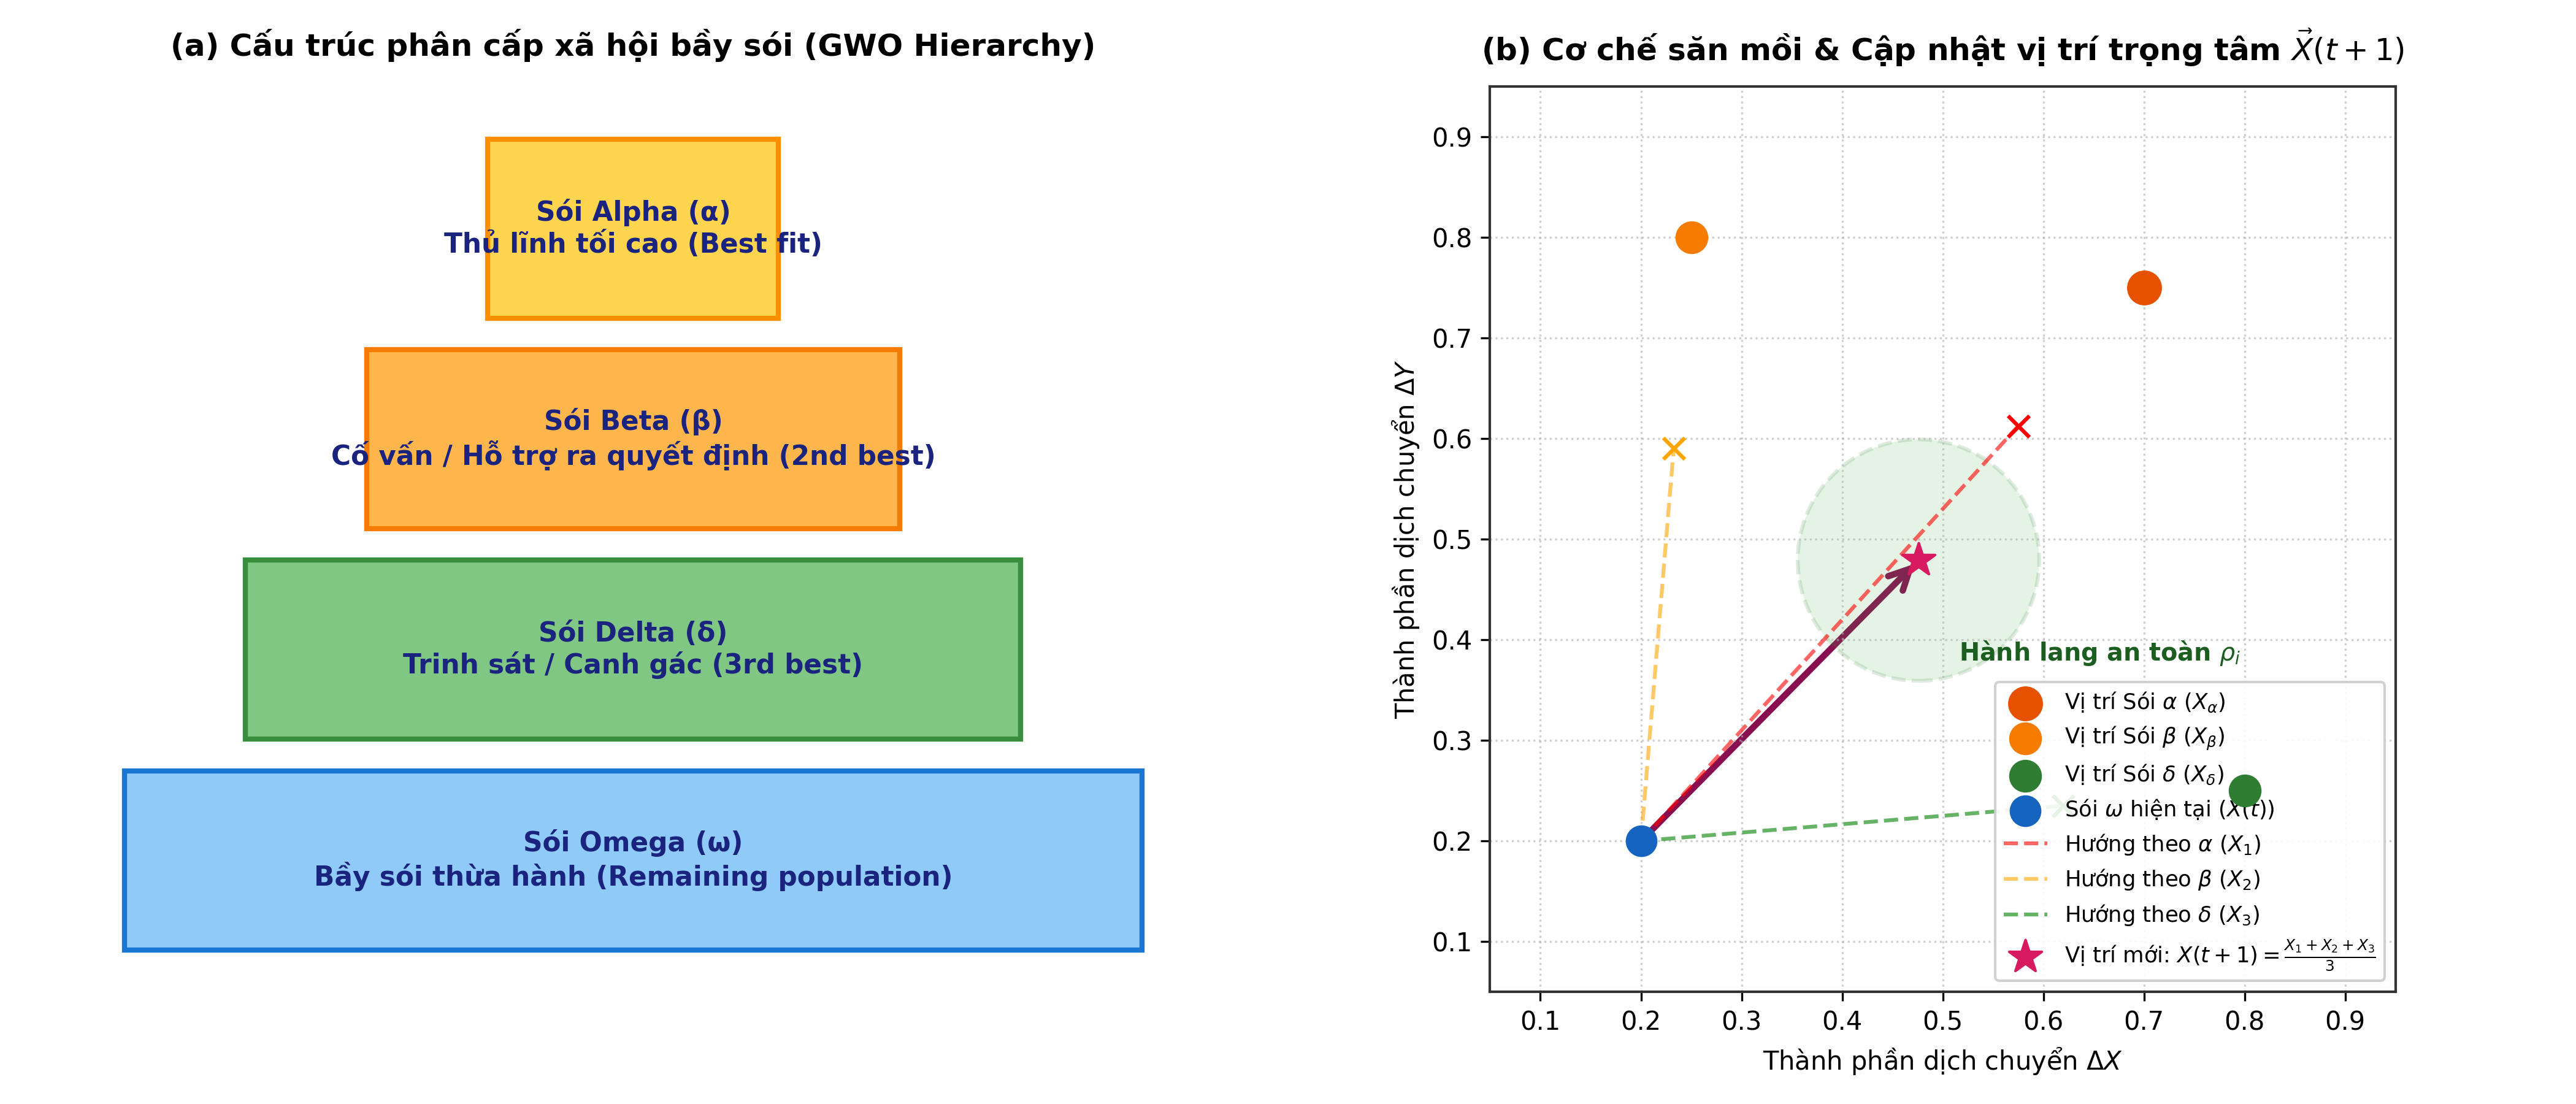
\includegraphics[width=\textwidth]{report_figures/fig_gwo_hierarchy_mechanism.png}
\caption{Thuật toán bầy sói xám: (a) Cấu trúc thứ bậc bầy đàn 4 cấp ($\alpha, \beta, \delta, \omega$); (b) Cách các cá thể cập nhật vị trí mới theo trọng tâm của ba con sói dẫn đầu bên trong hành lang an toàn.}
\label{fig:gwo_hierarchy_mechanism}
\end{figure}

Trong quá trình tìm kiếm, mỗi con sói sẽ tính toán 3 hướng dịch chuyển bám theo ba con sói đầu đàn ($\vec{X}_\alpha, \vec{X}_\beta, \vec{X}_\delta$):
\begin{align}
    \vec{D}_\alpha &= |\vec{C}_1 \cdot \vec{X}_\alpha - \vec{X}|, \quad \vec{X}_1 = \vec{X}_\alpha - \vec{A}_1 \cdot \vec{D}_\alpha \\
    \vec{D}_\beta  &= |\vec{C}_2 \cdot \vec{X}_\beta - \vec{X}|,  \quad \vec{X}_2 = \vec{X}_\beta - \vec{A}_2 \cdot \vec{D}_\beta \\
    \vec{D}_\delta &= |\vec{C}_3 \cdot \vec{X}_\delta - \vec{X}|, \quad \vec{X}_3 = \vec{X}_\delta - \vec{A}_3 \cdot \vec{D}_\delta
\end{align}

Vị trí mới của cá thể là trung bình cộng tọa độ của 3 hướng này:
\begin{equation}
    \vec{X}(t+1) = \frac{\vec{X}_1 + \vec{X}_2 + \vec{X}_3}{3}
\end{equation}

Hệ số co cụm $a = 2 - 2(t / t_{\max})$ giảm dần theo số vòng lặp giúp đàn sói lúc đầu phân tán rộng để tìm đường mới, càng về sau càng hội tụ sát quanh vị trí tối ưu nhất.

\section{Kết quả thử nghiệm và đánh giá chất lượng chuyển động}
\label{sec:benchmark_results}

Thuật toán được kiểm chứng trực tiếp trên mô phỏng tay máy Denso VS-6556 trong môi trường ROS 2 và Gazebo với bài toán di chuyển né 3 vật cản đặt trên bàn. Kết quả được so sánh đối đầu giữa phương pháp Bi-RRT gốc (đường gấp khúc $C^0$) và phương pháp đề xuất Bi-RRT kết hợp tối ưu bầy sói GWO (đường cong trơn $C^2$).

Hình dạng quỹ đạo thực tế trong không gian và đồ thị biến thiên độ giật Jerk theo thời gian được mô tả trong Hình~\ref{fig:trajectory_comparison_rrt_vs_gwo}.

\begin{figure}[htbp]
\centering
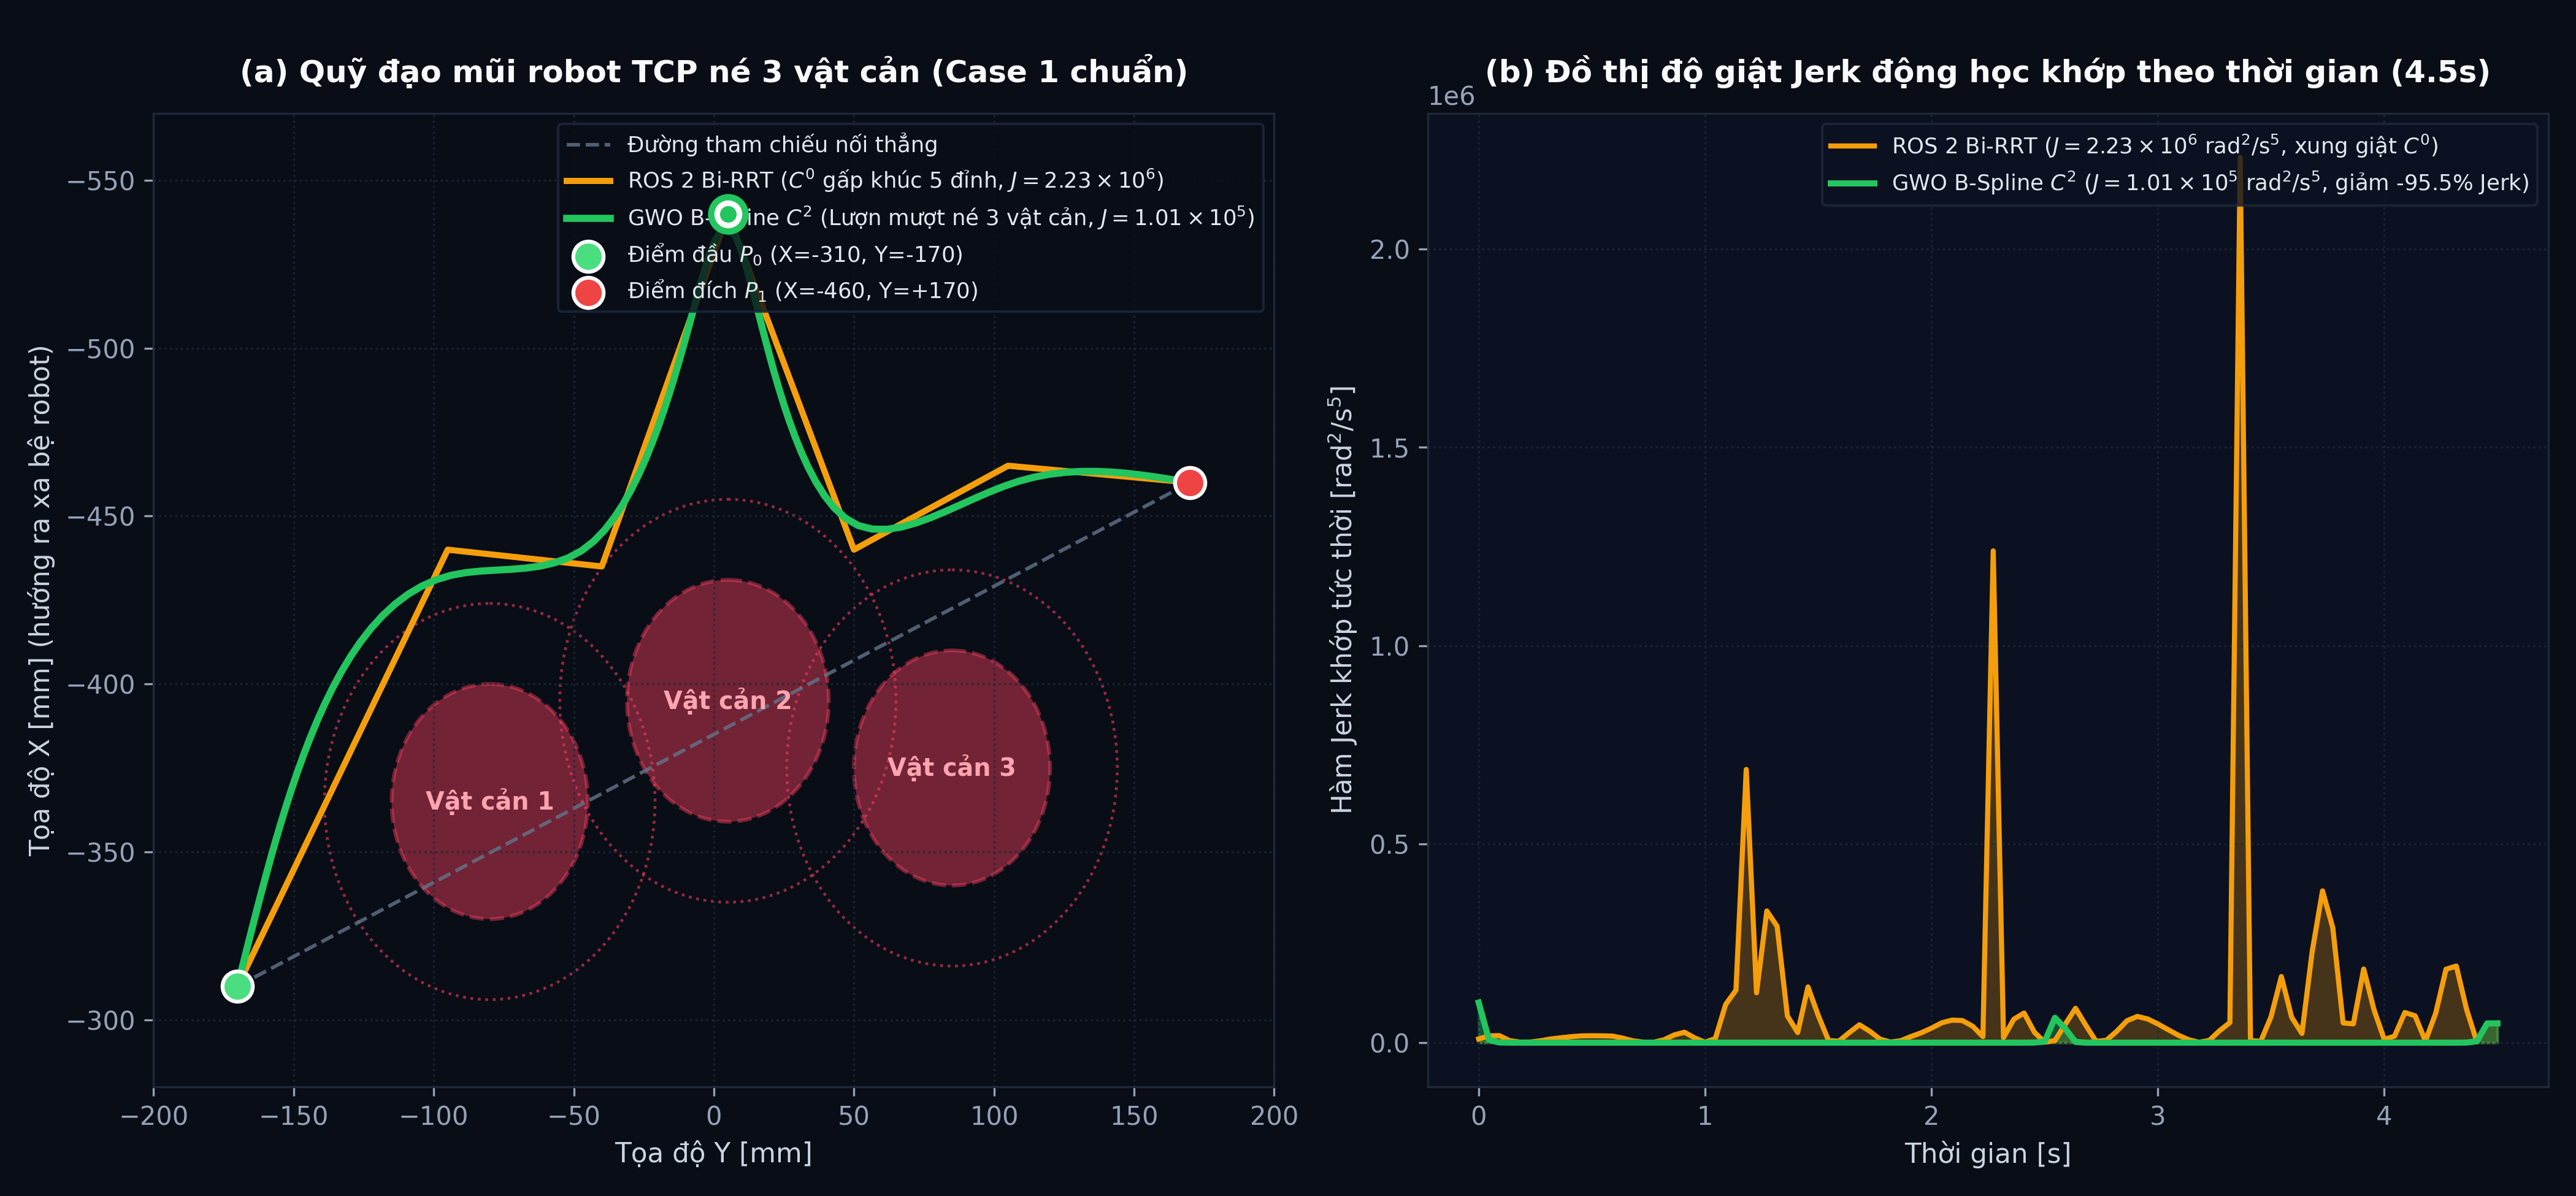
\includegraphics[width=\textwidth]{report_figures/fig_trajectory_comparison_rrt_vs_gwo.png}
\caption{So sánh chuyển động giữa phương pháp Bi-RRT gốc và phương pháp tối ưu bầy sói GWO: (a) Hình dạng quỹ đạo né 3 vật cản trên bàn làm việc; (b) Đồ thị độ giật Jerk của khớp tay máy theo thời gian.}
\label{fig:trajectory_comparison_rrt_vs_gwo}
\end{figure}

Bảng~\ref{tab:benchmark_metrics_nature} tổng hợp số liệu đo đạc cụ thể trên từng khớp của robot Denso VS-6556.

\begin{table}[htbp]
\centering
\caption{Bảng so sánh định lượng các chỉ số chất lượng giữa phương pháp gốc và phương pháp đề xuất}
\label{tab:benchmark_metrics_nature}
\resizebox{\textwidth}{!}{%
\begin{tabular}{lcccccc}
\toprule
\textbf{Khớp truyền động} & \textbf{Độ giật gốc} & \textbf{Độ giật GWO} & \textbf{Mức giảm giật} & \textbf{Năng lượng gốc} & \textbf{Năng lượng GWO} & \textbf{Mức tiết kiệm} \\
\midrule
Khớp 1 (Xoay đế)     & $2.03 \times 10^4$ & $1.62 \times 10^4$ & $-20.4\%$ & $56.8\text{ J}$  & $53.7\text{ J}$  & $-5.6\%$  \\
Khớp 2 (Nâng vai)    & $4.34 \times 10^5$ & $1.22 \times 10^4$ & $-97.2\%$ & $130.3\text{ J}$ & $87.8\text{ J}$  & $-32.6\%$ \\
Khớp 3 (Gập khuỷu)   & $1.46 \times 10^6$ & $4.71 \times 10^4$ & $-96.8\%$ & $203.8\text{ J}$ & $135.7\text{ J}$ & $-33.4\%$ \\
Khớp 4 (Cẳng tay)    & $2.20 \times 10^0$ & $2.03 \times 10^{-1}$ & $-90.8\%$ & $0.0\text{ J}$   & $0.0\text{ J}$   & $-38.0\%$ \\
Khớp 5 (Cổ tay)      & $3.00 \times 10^5$ & $1.12 \times 10^4$ & $-96.3\%$ & $3.0\text{ J}$   & $1.9\text{ J}$   & $-35.5\%$ \\
Khớp 6 (Mặt bích)    & $2.03 \times 10^4$ & $1.61 \times 10^4$ & $-20.8\%$ & $2.5\text{ J}$   & $2.4\text{ J}$   & $-5.6\%$  \\
\midrule
\textbf{TỔNG CỘNG}   & $\bm{2.23 \times 10^6}$ & $\bm{1.01 \times 10^5}$ & $\bm{-95.5\%}$ & $\bm{396.4\text{ J}}$ & $\bm{281.5\text{ J}}$ & $\bm{-29.0\%}$ \\
\bottomrule
\end{tabular}%
}
\end{table}

Các kết quả thử nghiệm cho thấy những cải thiện rõ rệt:

Về độ êm ái chuyển động, tổng độ giật động học giảm rất mạnh từ $2.23 \times 10^6$ xuống còn $1.01 \times 10^5\ \text{rad}^2/\text{s}^5$ (giảm tới $-95.5\%$). Các đỉnh giật góc tại khúc cua bị triệt tiêu hoàn toàn, giúp cánh tay robot di chuyển liên tục, không bị rung lắc.

Về mức tiêu hao năng lượng, tổng điện năng tiêu thụ của 6 cụm động cơ giảm từ $396.4\text{ J}$ xuống $281.5\text{ J}$ (tiết kiệm $-29.0\%$). Mức tiết kiệm này có được nhờ việc robot không phải liên tục phanh gấp rồi tăng tốc tại các khúc quanh nhọn.

Về độ an toàn di chuyển, robot luôn giữ khoảng cách an toàn tối thiểu trên $20\text{ mm}$ so với 3 vật cản trên bàn, không xảy ra va chạm hay hiện tượng vung tay nguy hiểm trong suốt quá trình thao tác.
